\documentclass[11pt,a4paper]{jsarticle}
\usepackage[dvips]{graphicx}
\usepackage{here}
\usepackage{longtable}
\usepackage{fancyhdr}
\setcounter{page}{0}
%
\begin{document}

\title{制御工学実験II \\ サーボモータのディジタル制御}
\author{提出者 \\ 14104064 下松八重 宏太 \\ \\ 共同実験者 \\ 14101028 梶野 翔平 \\ 14104092 中島 美香 \\ 16104311 北山 拓夢 \\ 13104119 廣瀬 直人}
\date{実験日 2016年7月4日 \\ 提出日 \today}



\maketitle
\thispagestyle{empty}
\newpage


\section{目的}
ディジタル計算機をコントローラとして用いる場合,ソフトウェアで制御則を実現できるので,アナログ制御と比べ制御則の修正・変更が容易である.ここではサーボモータのディジタル制御実験を通じて,ディジタル制御の理解を深める.
\section{原理}
今回の実験で用いる制御系の構成を図\ref{fig1}に示す.図中の変数の意味を表\ref{tab1}に示す.$T$をサンプリング周期とし,簡単のため,時刻$kT(k=0,1,2,\cdots)$でのみ値を持つ離散時間信号,及び連続時間信号の両方が存在する.したがって,ディジタル制御系では離散時間信号を連続時間信号に変換するサンプラと零次ホールド,及び連続時間信号を離散時間信号に変換するサンプラが必要になる.なお離散時間信号を連続時間信号に変換するサンプラと零次ホールドは式\ref{eq1}に示す通り,時刻$kT$で入力された離散時間信号を1サンプリング時間保持し,一定値の連続時間信号を出力する.
\begin{equation}
 u(t) = u(kT)\ \ (kT \le t \leq (k+1)T)
  \label{eq1}
\end{equation}

\begin{table}[b]
 \begin{center}
  \caption{制御系の各変数}
  \label{tab1}
  \begin{tabular}{|c|c|} \hline
   変数 & 意味 \\ \hline \hline
   $\Theta_d (k)$ & 目標角度(離散時間信号) \\ \hline
   $e(k)$         & 制御偏差(離散時間信号) \\ \hline
   $u(k)$         & 制御入力(離散時間信号) \\ \hline
   $u(t)$         & 制御入力(連続時間信号) \\ \hline
   $\theta (t)$   & 出力角度(連続時間信号) \\ \hline
   $\theta (k)$   & 制御出力(離散時間信号) \\ \hline
  \end{tabular}
 \end{center}
\end{table}

次に,この制御系のパルス伝達関数を求める.まず,$u(k),\theta (k)$の$z$変換をそれぞれ,$U(z) = Z[u(k)],\Theta (z) = Z[\theta (k)]$とすると,制御対象のパルス伝達関数は
\begin{eqnarray}
 G_p (z) & = & \frac{\Theta(z)}{U(z)} = Z[\frac{1-e^{-Ts}}{s} \frac{1}{s}] = (1-z^{-1})z[\frac{1}{s^2}] \nonumber \\ 
& = & \frac{T}{z-1}
\end{eqnarray}
となる.ここで,ディジタル計算機は制御入力を求めるための演算時間を必要とする.すなわち時刻$kT$の制御偏差時刻$e(kT)$を用いて求めた制御入力$u(kT)$は,実際には時刻$(k+1)T$に制御対象に入力される.この演算時間遅れを考え,制御対象のパルス伝達関数を次式に示す.
\begin{equation}
 G_p (z) = \frac{\Theta(z)}{U(z)} = \frac{T}{z^2-z}
\end{equation}
制御系のブロック線図を図\ref{fig2}に示す.図\ref{fig2}より,制御系のパルス伝達関数は
\begin{equation}
 G(z) = \frac{\Theta(z)}{\Theta_d (z)} = \frac{gT}{z^2-z+gT}
\label{eq4}
\end{equation}
となり,その極を$P_i (i = 1,2)$とすると,$|P_i| < 1$,すなわち
\begin{equation}
 0 < g < \frac{1}{T}
\label{eq5}
\end{equation}
であれば制御系は漸近安定となる.

\section{実験方法}
定数ゲイン$g = 1.0,2.1$として制御プログラムに定常ゲインを入力する.サンプリング周期を$0.02,0.1,0.5[s]$としてそれぞれの場合で実験を行う.目標角度は$60$[deg]とする.

\section{結果と考察}
実験結果を表\ref{tab2}から表\ref{tab7},図\ref{fig3}から図\ref{fig8}に示す.

\begin{longtable}[c]{|c|c|c|c|}
  \caption{定数ゲイン1.0,サンプリング周期0.02[s]のときの実験結果}
  \label{tab2} \\
  \hline
   時間& 	入力電圧[V]&	出力角度[deg]&	目標角度[deg] \\ \hline \hline \endfirsthead 
\hline \endhead
\hline \endfoot
\hline \endlastfoot
   0   & 	0    &  0.00  &  60 \\ \hline 
   0.1 & 	1.51 & 	7.44  &  60 \\ \hline 
   0.2 & 	1.28 & 	15.6  & 60  \\ \hline 
   0.3 & 	1.08 & 	22.44 & 60  \\ \hline 
   0.4 & 	0.91 & 	28.19 & 60  \\ \hline 
   0.5 & 	0.77 & 	33.11 & 60  \\ \hline 
   0.6 & 	0.65 & 	37.25 & 60  \\ \hline 
   0.7 & 	0.55 & 	40.73 & 60  \\ \hline 
   0.8 & 	0.47 & 	43.73 & 60  \\ \hline 
   0.9 & 	0.4  & 	46.19 & 60  \\ \hline 
   1   & 	0.34 & 	48.29 & 60  \\ \hline 
   1.1 & 	0.28 & 	50.09 & 60  \\ \hline 
   1.2 & 	0.24 & 	51.59 & 60  \\ \hline 
   1.3 & 	0.2  & 	52.91 & 60  \\ \hline 
   1.4 & 	0.17 & 	53.99 & 60  \\ \hline 
   1.5 & 	0.15 & 	54.89 & 60  \\ \hline 
   1.6 & 	0.12 & 	55.67 & 60  \\ \hline 
   1.7 & 	0.11 & 	56.33 & 60  \\ \hline 
   1.8 & 	0.09 & 	56.87 & 60  \\ \hline 
   1.9 & 	0.08 & 	57.35 & 60  \\ \hline 
   2   & 	0.06 & 	57.77 & 60  \\ \hline 
   2.1 & 	0.05 & 	58.13 & 60  \\ \hline 
   2.2 & 	0.05 & 	58.37 & 60  \\ \hline 
   2.3 & 	0.04 & 	58.61 & 60  \\ \hline 
   2.4 & 	0.03 & 	58.85 & 60  \\ \hline 
   2.5 & 	0.03 & 	58.97 & 60  \\ \hline 
   2.6 & 	0.03 & 	59.15 & 60  \\ \hline 
   2.7 & 	0.02 & 	59.27 & 60  \\ \hline 
   2.8 & 	0.02 & 	59.33 & 60  \\ \hline 
   2.9 & 	0.02 & 	59.45 & 60  \\ \hline 
   3   & 	0.01 & 	59.51 & 60  \\ \hline 
   3.1 & 	0.01 & 	59.57 & 60  \\ \hline 
   3.2 & 	0.01 & 	59.63 & 60  \\ \hline 
   3.3 & 	0.01 & 	59.69 & 60  \\ \hline 
   3.4 & 	0.01 & 	59.69 & 60  \\ \hline 
   3.5 & 	0.01 & 	59.75 & 60  \\ \hline 
   3.6 & 	0.01 & 	59.75 & 60  \\ \hline 
   3.7 & 	0.01 & 	59.81 & 60  \\ \hline 
   3.8 & 	0.01 & 	59.81 & 60  \\ \hline 
   3.9 & 	0    & 	59.87 & 60  \\ \hline 
   4   & 	0    & 	59.87 & 60  \\ \hline 
   4.1 & 	0    & 	59.87 & 60  \\ \hline 
   4.2 & 	0    & 	59.87 & 60  \\ \hline 
   4.3 & 	0    & 	59.87 & 60  \\ \hline 
   4.4 & 	0    & 	59.87 & 60  \\ \hline 
   4.5 & 	0    & 	59.87 & 60  \\ \hline 
   4.6 & 	0    & 	59.87 & 60  \\ \hline 
   4.7 & 	0    & 	59.87 & 60  \\ \hline 
   4.8 & 	0    & 	59.87 & 60  \\ \hline 
   4.9 & 	0    & 	59.87 & 60  \\ \hline 
   5   & 	0    & 	59.87 & 60  \\ \hline 
   5.1 & 	0    & 	59.87 & 60  \\ \hline 
   5.2 & 	0    & 	59.87 & 60  \\ \hline 
   5.3 & 	0    & 	59.87 & 60  \\ \hline 
   5.4 & 	0    & 	59.87 & 60  \\ \hline 
   5.5 & 	0    & 	59.87 & 60  \\ \hline 
   5.6 & 	0    & 	59.87 & 60  \\ \hline 
   5.7 & 	0    & 	59.87 & 60  \\ \hline 
   5.8 & 	0    & 	59.87 & 60  \\ \hline 
   5.9 & 	0    & 	59.87 & 60  \\ \hline 
  \end{longtable}

\begin{longtable}[c]{|c|c|c|c|}
  \caption{定数ゲイン1.0,サンプリング周期0.1[s]のときの実験結果}
  \label{tab3} \\
  \hline
   時間& 	入力電圧[V]&	出力角度[deg]&	目標角度[deg] \\ \hline \hline \endfirsthead 
\hline \endhead
\hline \endfoot
\hline \endlastfoot
時間& 	入力電圧[V]&    出力角度[deg]&	目標角度[deg] \\ \hline
0   & 	0    & 0      & 	60 \\ \hline 
0.1 & 	1.67 & 	0     & 	60 \\ \hline 
0.2 & 	1.67 & 	9.84  & 	60 \\ \hline 
0.3 & 	1.39 & 	19.8  & 	60 \\ \hline 
0.4 & 	1.12 & 	28.01 & 	60 \\ \hline 
0.5 & 	0.89 & 	34.67 & 	60 \\ \hline 
0.6 & 	0.7  & 	39.95 & 	60 \\ \hline 
0.7 & 	0.56 & 	44.15 & 	60 \\ \hline 
0.8 & 	0.44 & 	47.45 & 	60 \\ \hline 
0.9 & 	0.35 & 	50.03 & 	60 \\ \hline 
1   & 	0.28 & 	52.13 & 	60 \\ \hline 
1.1 & 	0.22 & 	53.75 & 	60 \\ \hline 
1.2 & 	0.17 & 	55.01 & 	60 \\ \hline 
1.3 & 	0.14 & 	56.03 & 	60 \\ \hline 
1.4 & 	0.11 & 	56.87 & 	60 \\ \hline 
1.5 & 	0.09 & 	57.53 & 	60 \\ \hline 
1.6 & 	0.07 & 	58.01 & 	60 \\ \hline 
1.7 & 	0.06 & 	58.43 & 	60 \\ \hline 
1.8 & 	0.04 & 	58.73 & 	60 \\ \hline 
1.9 & 	0.04 & 	58.97 & 	60 \\ \hline 
2   & 	0.03 & 	59.15 & 	60 \\ \hline 
2.1 & 	0.02 & 	59.33 & 	60 \\ \hline 
2.2 & 	0.02 & 	59.45 & 	60 \\ \hline 
2.3 & 	0.02 & 	59.51 & 	60 \\ \hline 
2.4 & 	0.01 & 	59.63 & 	60 \\ \hline 
2.5 & 	0.01 & 	59.69 & 	60 \\ \hline 
2.6 & 	0.01 & 	59.75 & 	60 \\ \hline 
2.7 & 	0.01 & 	59.75 & 	60 \\ \hline 
2.8 & 	0.01 & 	59.81 & 	60 \\ \hline 
2.9 & 	0.01 & 	59.81 & 	60 \\ \hline 
3   & 	0.01 & 	59.87 & 	60 \\ \hline 
3.1 & 	0    & 	59.87 & 	60 \\ \hline 
3.2 & 	0    & 	59.87 & 	60 \\ \hline 
3.3 & 	0    & 	59.87 & 	60 \\ \hline 
3.4 & 	0    & 	59.87 & 	60 \\ \hline 
3.5 & 	0    & 	59.87 & 	60 \\ \hline 
3.6 & 	0    & 	59.87 & 	60 \\ \hline 
3.7 & 	0    & 	59.87 & 	60 \\ \hline 
3.8 & 	0    & 	59.87 & 	60 \\ \hline 
3.9 & 	0    & 	59.87 & 	60 \\ \hline 
4   & 	0    & 	59.87 & 	60 \\ \hline 
4.1 & 	0    & 	59.87 & 	60 \\ \hline 
4.2 & 	0    & 	59.87 & 	60 \\ \hline 
4.3 & 	0    & 	59.87 & 	60 \\ \hline 
4.4 & 	0    & 	59.87 & 	60 \\ \hline 
4.5 & 	0    & 	59.87 & 	60 \\ \hline 
4.6 & 	0    & 	59.87 & 	60 \\ \hline 
4.7 & 	0    & 	59.87 & 	60 \\ \hline 
4.8 & 	0    & 	59.87 & 	60 \\ \hline 
4.9 & 	0    & 	59.87 & 	60 \\ \hline 
5   & 	0    & 	59.87 & 	60 \\ \hline 
5.1 & 	0    & 	59.87 & 	60 \\ \hline 
5.2 & 	0    & 	59.87 & 	60 \\ \hline 
5.3 & 	0    & 	59.87 & 	60 \\ \hline 
5.4 & 	0    & 	59.87 & 	60 \\ \hline 
5.5 & 	0    & 	59.87 & 	60 \\ \hline 
5.6 & 	0    & 	59.87 & 	60 \\ \hline 
5.7 & 	0    & 	59.87 & 	60 \\ \hline 
5.8 & 	0    & 	59.87 & 	60 \\ \hline 
5.9 & 	0    & 	59.87 & 	60 \\ \hline 

  \end{longtable}


\begin{longtable}[c]{|c|c|c|c|}
  \caption{定数ゲイン1.0,サンプリング周期0.5[s]のときの実験結果}
  \label{tab4} \\
  \hline
   時間& 	入力電圧[V]&	出力角度[deg]&	目標角度[deg] \\ \hline \hline \endfirsthead 
\hline \endhead
\hline \endfoot
\hline \endlastfoot
時間& 	入力電圧[V]&    出力角度[deg]&	目標角度[deg] \\ \hline
0   & 	0    & 	0      &60 \\ \hline 
0.5 &	1.67 &	0      &60 \\ \hline 
1   &	1.67 &	49.67  &60 \\ \hline 
1.5 &	0.29 &	99.46  &60 \\ \hline 
2   &	-1.1 &	107.98 &60 \\ \hline 
2.5 &	-1.33&	74.99  &60 \\ \hline 
3   &	-0.42&	34.91  &60 \\ \hline 
3.5 &	0.7  &	22.32  &60 \\ \hline 
4   &	1.05 &	42.89  &60 \\ \hline 
4.5 &	0.48 &	74.09  &60 \\ \hline 
5   &	-0.39&	88.3   &60 \\ \hline 
5.5 &	-0.79&	76.49  &60 \\ \hline 
6   &	-0.46&	52.67  &60 \\ \hline 
6.5 &	0.2  &	38.87  &60 \\ \hline 
7   &	0.59 &	44.81  &60 \\ \hline 
7.5 &	0.42 &	62.33  &60 \\ \hline 
8   &	-0.06&	74.87  &60 \\ \hline 
8.5 &	-0.41&	72.89  &60 \\ \hline 
9   &	-0.36&	60.41  &60 \\ \hline 
9.5 &	-0.01&	49.55  &60 \\ \hline 
10  &	0.29 &	49.13  &60 \\ \hline 
10.5&	0.3  &	57.65  &60 \\ \hline 
11  &	0.07 &	66.59  &60 \\ \hline 
11.5&	-0.18&	68.51  &60 \\ \hline 
12  &	-0.24&	62.99  &60 \\ \hline 
12.5&	-0.08&	55.73  &60 \\ \hline 
13  &	0.12 &	53.09  &60 \\ \hline 
13.5&	0.19 &	56.51  &60 \\ \hline 
14  &	0.1  &	62.27  &60 \\ \hline 
14.5&	-0.06&	65.03  &60 \\ \hline 
15  &	-0.14&	63.17  &60 \\ \hline 
15.5&	-0.09&	58.91  &60 \\ \hline 
16  &	0.03 &	56.15  &60 \\ \hline 
16.5&	0.11 &	56.93  &60 \\ \hline 
17  &	0.09 &	60.05  &60 \\ \hline 
17.5&	0    &	62.45  &60 \\ \hline 
18  &	-0.07&	60.23  &60 \\ \hline 
18.5&	-0.07&	58.19  &60 \\ \hline 
19  &	-0.01&	57.89  &60 \\ \hline 
19.5&	0.05 &	59.33  &60 \\ \hline 
20  &	0.06 &	61.07  &60 \\ \hline 
20.5&	0.02 &	61.49  &60 \\ \hline 
21  &	-0.03&	60.53  &60 \\ \hline 
21.5&	-0.04&	59.21  &60 \\ \hline 
22  &	-0.01&	58.61  &60 \\ \hline 
22.5&	0.02 &	59.15  &60 \\ \hline 
23  &	0.04 &	60.17  &60 \\ \hline 
23.5&	0.03 &	60.77  &60 \\ \hline 
24  &	0    &	60.71  &60 \\ \hline 
24.5&	-0.02&	59.99  &60 \\ \hline 
25  &	-0.02&	59.21  &60 \\ \hline 
25.5&	0    &	59.21  &60 \\ \hline 
26  &	0.02 &	59.75  &60 \\ \hline 
26.5&	0.02 &	60.35  &60 \\ \hline 
27  &	0.01 &	60.53  &60 \\ \hline 
27.5&	-0.01&	60.29  &60 \\ \hline 
28  &	-0.01&	59.69  &60 \\ \hline 
28.5&	-0.01&	59.39  &60 \\ \hline 
29  &	0.01 &	59.51  &60 \\ \hline 
29.5&	0.02 &	59.51  &60 \\ \hline 

\end{longtable}
\begin{longtable}[c]{|c|c|c|c|}
  \caption{定数ゲイン2.1,サンプリング周期0.02[s]のときの実験結果}
  \label{tab5} \\
  \hline
   時間& 	入力電圧[V]&	出力角度[deg]&	目標角度[deg] \\ \hline \hline \endfirsthead 
\hline \endhead
\hline \endfoot
\hline \endlastfoot
時間& 	入力電圧[V]&    出力角度[deg]&	目標角度[deg] \\ \hline
0   & 	0    & 	0     &	60 \\ \hline 
0.1 &	2.84 &	14.76 &	60 \\ \hline 
0.2 &	1.95 &	28.91 &	60 \\ \hline 
0.3 &	1.34 &	38.63 &	60 \\ \hline 
0.4 &	0.92 &	45.29 &	60 \\ \hline 
0.5 &	0.64 &	49.85 &	60 \\ \hline 
0.6 &	0.44 &	53.03 &	60 \\ \hline 
0.7 &	0.3  &	55.19 &	60 \\ \hline 
0.8 &	0.21 &	56.69 &	60 \\ \hline 
0.9 &	0.14 &	57.71 &	60 \\ \hline 
1   &	0.1  &	58.43 &	60 \\ \hline 
1.1 &	0.07 &	58.91 &	60 \\ \hline 
1.2 &	0.05 &	59.27 &	60 \\ \hline 
1.3 &	0.03 &	59.45 &	60 \\ \hline 
1.4 &	0.03 &	59.63 &	60 \\ \hline 
1.5 &	0.02 &	59.75 &	60 \\ \hline 
1.6 &	0.01 &	59.81 &	60 \\ \hline 
1.7 &	0.01 &	59.87 &	60 \\ \hline 
1.8 &	0.01 &	59.87 &	60 \\ \hline 
1.9 &	0    &	59.93 &	60 \\ \hline 
2   &	0    &	59.93 &	60 \\ \hline 
2.1 &	0    &	59.93 &	60 \\ \hline 
2.2 &	0    &	59.93 &	60 \\ \hline 
2.3 &	0    &	59.93 &	60 \\ \hline 
2.4 &	0    &	59.93 &	60 \\ \hline 
2.5 &	0    &	59.93 &	60 \\ \hline 
2.6 &	0    &	59.93 &	60 \\ \hline 
2.7 &	0    &	59.93 &	60 \\ \hline 
2.8 &	0    &	59.93 &	60 \\ \hline 
2.9 &	0    &	59.93 &	60 \\ \hline 
3   &	0    &	59.93 &	60 \\ \hline 
3.1 &	0    &	59.93 &	60 \\ \hline 
3.2 &	0    &	59.93 &	60 \\ \hline 
3.3 &	0    &	59.93 &	60 \\ \hline 
3.4 &	0    &	59.93 &	60 \\ \hline 
3.5 &	0    &	59.93 &	60 \\ \hline 
3.6 &	0    &	59.93 &	60 \\ \hline 
3.7 &	0    &	59.93 &	60 \\ \hline 
3.8 &	0    &	59.93 &	60 \\ \hline 
3.9 &	0    &	59.93 &	60 \\ \hline 
4   &	0    &	59.93 &	60 \\ \hline 
4.1 &	0    &	59.93 &	60 \\ \hline 
4.2 &	0    &	59.93 &	60 \\ \hline 
4.3 &	0    &	59.93 &	60 \\ \hline 
4.4 &	0    &	59.93 &	60 \\ \hline 
4.5 &	0    &	59.93 &	60 \\ \hline 
4.6 &	0    &	59.93 &	60 \\ \hline 
4.7 &	0    &	59.93 &	60 \\ \hline 
4.8 &	0    &	59.93 &	60 \\ \hline 
4.9 &	0    &	59.93 &	60 \\ \hline 
5   &	0    &	59.93 &	60 \\ \hline 
5.1 &	0    &	59.93 &	60 \\ \hline 
5.2 &	0    &	59.93 &	60 \\ \hline 
5.3 &	0    &	59.93 &	60 \\ \hline 
5.4 &	0    &	59.93 &	60 \\ \hline 
5.5 &	0    &	59.93 &	60 \\ \hline 
5.6 &	0    &	59.93 &	60 \\ \hline 
5.7 &	0    &	59.93 &	60 \\ \hline 
5.8 &	0    &	59.93 &	60 \\ \hline 
5.9 &	0    &	59.93 &	60 \\ \hline 
\end{longtable}



\begin{longtable}[c]{|c|c|c|c|}
  \caption{定数ゲイン2.1,サンプリング周期0.1[s]のときの実験結果}
  \label{tab6} \\
  \hline
   時間& 	入力電圧[V]&	出力角度[deg]&	目標角度[deg] \\ \hline \hline \endfirsthead 
\hline \endhead
\hline \endfoot
\hline \endlastfoot
時間& 	入力電圧[V]&    出力角度[deg]&	目標角度[deg] \\ \hline
0   &	0    &	0     &	60 \\ \hline 
0.1 &	3.5  &	0     &	60 \\ \hline 
0.2 &	3.5  &	20.4  &	60 \\ \hline 
0.3 &	2.31 &	41.27 &	60 \\ \hline 
0.4 &	1.09 &	55.01 &	60 \\ \hline 
0.5 &	0.29 &	61.55 &	60 \\ \hline 
0.6 &	-0.09&	63.29 &	60 \\ \hline 
0.7 &	-0.19&	62.81 &	60 \\ \hline 
0.8 &	-0.16&	61.61 &	60 \\ \hline 
0.9 &	-0.09&	60.59 &	60 \\ \hline 
1   &	-0.03&	60.05 &	60 \\ \hline 
1.1 &	0    &	59.81 &	60 \\ \hline 
1.2 &	0.01 &	59.75 &	60 \\ \hline 
1.3 &	0.01 &	59.81 &	60 \\ \hline 
1.4 &	0.01 &	59.81 &	60 \\ \hline 
1.5 &	0.01 &	59.87 &	60 \\ \hline 
1.6 &	0.01 &	59.93 &	60 \\ \hline 
1.7 &	0    &	59.99 &	60 \\ \hline 
1.8 &	0    &	59.99 &	60 \\ \hline 
1.9 &	0    &	59.99 &	60 \\ \hline 
2   &	0    &	59.99 &	60 \\ \hline 
2.1 &	0    &	59.99 &	60 \\ \hline 
2.2 &	0    &	59.99 &	60 \\ \hline 
2.3 &	0    &	59.99 &	60 \\ \hline 
2.4 &	0    &	59.99 &	60 \\ \hline 
2.5 &	0    &	59.99 &	60 \\ \hline 
2.6 &	0    &	59.99 &	60 \\ \hline 
2.7 &	0    &	59.99 &	60 \\ \hline 
2.8 &	0    &	59.99 &	60 \\ \hline 
2.9 &	0    &	59.99 &	60 \\ \hline 
3   &	0    &	59.99 &	60 \\ \hline 
3.1 &	0    &	59.99 &	60 \\ \hline 
3.2 &	0    &	59.99 &	60 \\ \hline 
3.3 &	0    &	59.99 &	60 \\ \hline 
3.4 &	0    &	59.99 &	60 \\ \hline 
3.5 &	0    &	59.99 &	60 \\ \hline 
3.6 &	0    &	59.99 &	60 \\ \hline 
3.7 &	0    &	59.99 &	60 \\ \hline 
3.8 &	0    &	59.99 &	60 \\ \hline 
3.9 &	0    &	59.99 &	60 \\ \hline 
4   &	0    &	59.99 &	60 \\ \hline 
4.1 &	0    &	59.99 &	60 \\ \hline 
4.2 &	0    &	59.99 &	60 \\ \hline 
4.3 &	0    &	59.99 &	60 \\ \hline 
4.4 &	0    &	59.99 &	60 \\ \hline 
4.5 &	0    &	59.99 &	60 \\ \hline 
4.6 &	0    &	59.99 &	60 \\ \hline 
4.7 &	0    &	59.99 &	60 \\ \hline 
4.8 &	0    &	59.99 &	60 \\ \hline 
4.9 &	0    &	59.99 &	60 \\ \hline 
5   &	0    &	59.99 &	60 \\ \hline 
5.1 &	0    &	59.99 &	60 \\ \hline 
5.2 &	0    &	59.99 &	60 \\ \hline 
5.3 &	0    &	59.99 &	60 \\ \hline 
5.4 &	0    &	59.99 &	60 \\ \hline 
5.5 &	0    &	59.99 &	60 \\ \hline 
5.6 &	0    &	59.99 &	60 \\ \hline 
5.7 &	0    &	59.99 &	60 \\ \hline 
5.8 &	0    &	59.99 &	60 \\ \hline 
5.9 &	0    &	59.99 &	60 \\ \hline 
\end{longtable}





\begin{longtable}[c]{|c|c|c|c|}
  \caption{定数ゲイン2.1,サンプリング周期0.5[s]のときの実験結果}
  \label{tab7} \\
  \hline
   時間& 	入力電圧[V]&	出力角度[deg]&	目標角度[deg] \\ \hline \hline \endfirsthead 
\hline \endhead
\hline \endfoot
\hline \endlastfoot
時間& 	入力電圧[V]&    出力角度[deg]&	目標角度[deg] \\ \hline
0   & 	0     &	0      &60 \\ \hline 
0.5 &	3.5   &	0.06   &60 \\ \hline 
1   &	3.5   &	103.96 &60 \\ \hline 
1.5 &	-2.56 &	208.28 &60 \\ \hline 
2   &	-5    &	132.75 &60 \\ \hline 
2.5 &	-4.24 &	-17.22 &60 \\ \hline 
3   &	4.5   &	-145.11&60 \\ \hline 
3.5 &	4.9   &	-14.58 &60 \\ \hline 
4   &	4.35  &	131.8  &60 \\ \hline 
4.5 &	-4.19 &	261.61 &60 \\ \hline 
5   &	-5    &	139.29 &60 \\ \hline 
5.5 &	-4.63 &	-10.86 &60 \\ \hline 
6   &	4.13  &	-150.27&60 \\ \hline 
6.5 &	4.9   &	-30.77 &60 \\ \hline 
7   &	4.9   &	115.66 &60 \\ \hline 
7.5 &	-3.25 &	261.91 &60 \\ \hline 
8   &	-5    &	167.43 &60 \\ \hline 
8.5 &	-5    &	17.34  &60 \\ \hline 
9   &	2.49  &	-133.17&60 \\ \hline 
9.5 &	4.9   &	-61.61 &60 \\ \hline 
10  &	4.9   &	84.82  &60 \\ \hline 
10.5&	-1.45 &	230.96 &60 \\ \hline 
11  &	-5    &	189.14 &60 \\ \hline 
11.5&	-5    &	39.47  &60 \\ \hline 
12  &	1.2   &	-111.04&60 \\ \hline 
12.5&	4.9   &	-76.97 &60 \\ \hline 
13  &	4.9   &	69.11  &60 \\ \hline 
13.5&	-0.53 &	215.18 &60 \\ \hline 
14  &	-5    &	200.42 &60 \\ \hline 
14.5&	-5    &	51.11  &60 \\ \hline 
15  &	0.52  &	-99.34 &60 \\ \hline 
15.5&	4.9   &	-85.18 &60 \\ \hline 
16  &	4.9   &	60.41  &60 \\ \hline 
16.5&	-0.02 &	206.54 &60 \\ \hline 
17  &	-5    &	206.78 &60 \\ \hline 
17.5&	-5    &	57.95  &60 \\ \hline 
18  &	0.12  &	-92.44 &60 \\ \hline 
18.5&	4.9   &	-90.04 &60 \\ \hline 
19  &	4.9   &	55.37  &60 \\ \hline 
19.5&	0.27  &	201.44 &60 \\ \hline 
20  &	-5    &	210.32 &60 \\ \hline 
20.5&	-5    &	61.67  &60 \\ \hline 
21  &	-0.1  &	-89.02 &60 \\ \hline 
21.5&	4.9   &	-92.86 &60 \\ \hline 
22  &	4.9   &	52.37  &60 \\ \hline 
22.5&	0.45  &	198.38 &60 \\ \hline 
23  &	-5    &	212.42 &60 \\ \hline 
23.5&	-5    &	63.89  &60 \\ \hline 
24  &	-0.23 &	-86.8  &60 \\ \hline 
24.5&	4.9   &	-94.54 &60 \\ \hline 
25  &	4.9   &	50.75  &60 \\ \hline 
25.5&	0.54  &	196.82 &60 \\ \hline 
26  &	-5    &	213.56 &60 \\ \hline 
26.5&	-5    &	65.03  &60 \\ \hline 
27  &	-0.29 &	-85.36 &60 \\ \hline 
27.5&	4.9   &	-95.14 &60 \\ \hline 
28  &	4.9   &	49.73  &60 \\ \hline 
28.5&	0.6   &	195.8  &60 \\ \hline 
29  &	-5    &	214.28 &60 \\ \hline 
29.5&	-5    &	65.81  &60 \\ \hline 
\end{longtable}









\begin{figure}[H]
 \begin{center}
  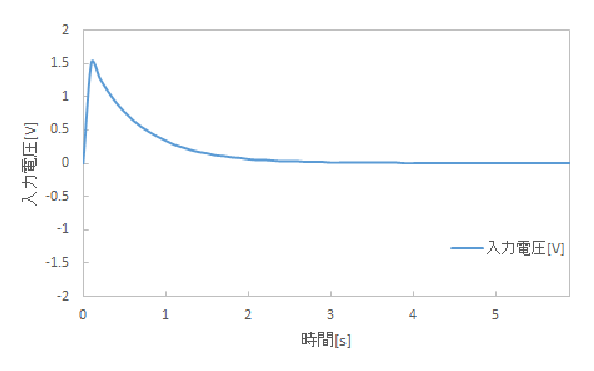
\includegraphics[scale=.6]{./picture/graph2.eps} \\
  (a)入力電圧 \\
  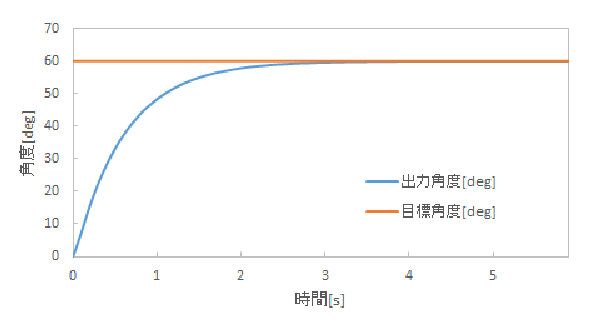
\includegraphics[scale=.6]{./picture/graph1.eps} \\
  (b)角度
  \caption{定数ゲイン1.0,サンプリング周期0.02[s]のときの実験結果}
  \label{fig3}
 \end{center}
\end{figure}

\begin{figure}[H]
 \begin{center}
  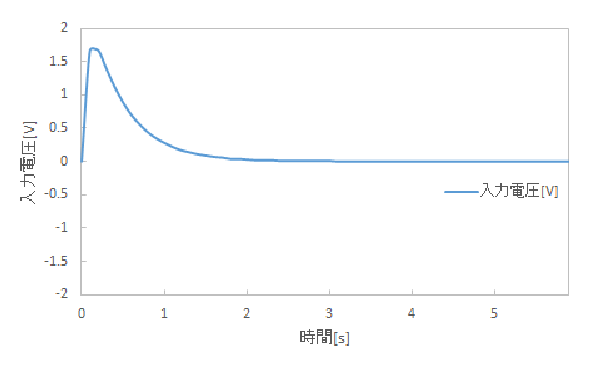
\includegraphics[scale=.6]{./picture/graph3.eps} \\
  (a)入力電圧 \\
  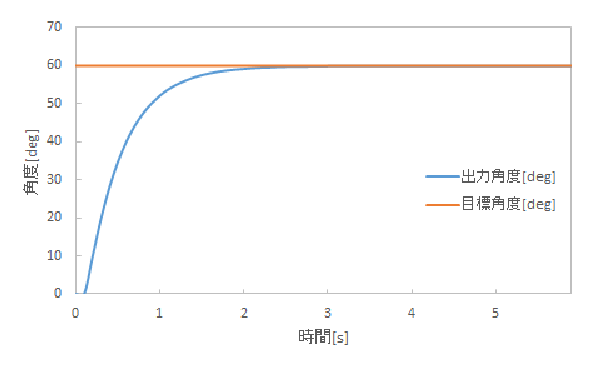
\includegraphics[scale=.6]{./picture/graph4.eps} \\
  (b)角度
  \caption{定数ゲイン1.0,サンプリング周期0.1[s]のときの実験結果}
  \label{fig4}
 \end{center}
\end{figure}

\begin{figure}[H]
 \begin{center}
  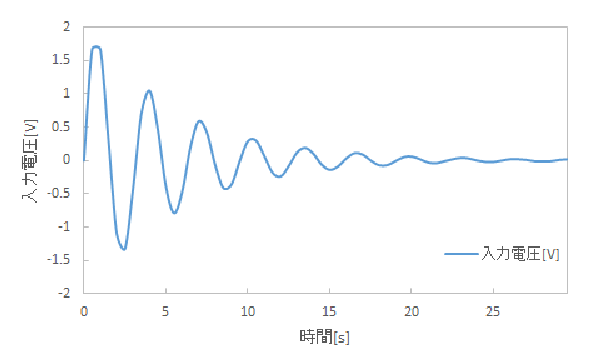
\includegraphics[scale=.6]{./picture/graph5.eps} \\
  (a)入力電圧 \\
  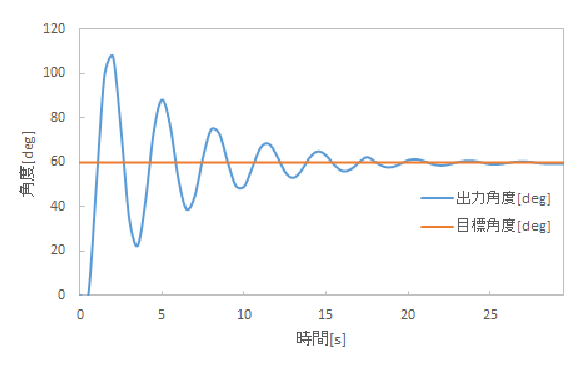
\includegraphics[scale=.6]{./picture/graph6.eps} \\
  (b)角度
  \caption{定数ゲイン1.0,サンプリング周期0.5[s]のときの実験結果}
  \label{fig5}
 \end{center}
\end{figure}

\begin{figure}[H]
 \begin{center}
  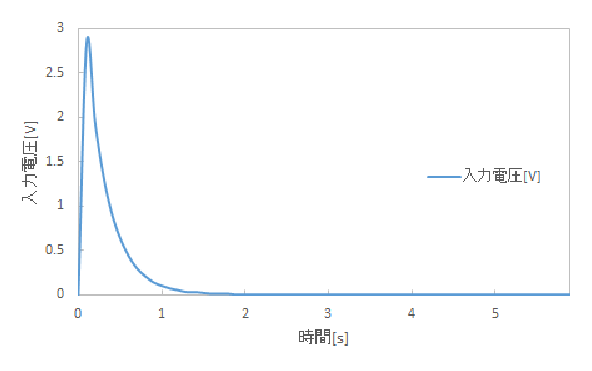
\includegraphics[scale=.6]{./picture/graph7.eps} \\
  (a)入力電圧 \\
  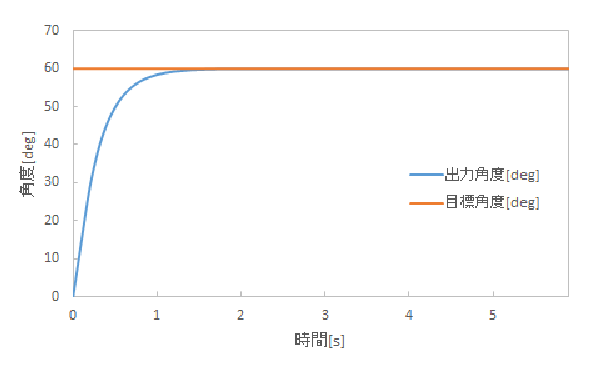
\includegraphics[scale=.7]{./picture/graph8.eps} \\
  (b)角度
  \caption{定数ゲイン2.1,サンプリング周期0.02[s]のときの実験結果}
  \label{fig6}
 \end{center}
\end{figure}

\begin{figure}[H]
 \begin{center}
  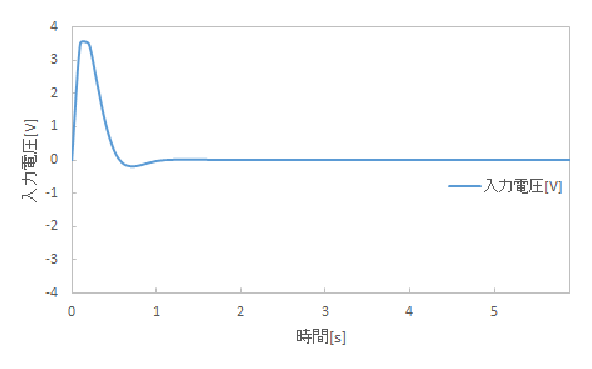
\includegraphics[scale=.6]{./picture/graph9.eps} \\
  (a)入力電圧 \\
  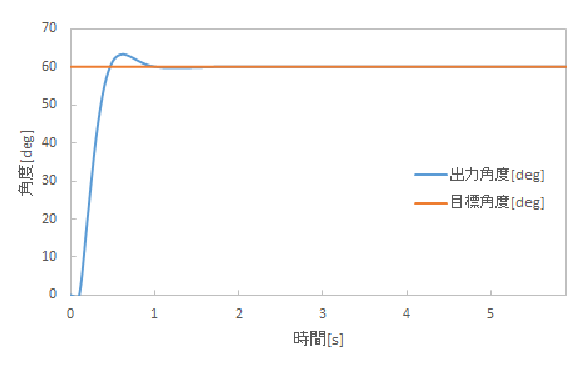
\includegraphics[scale=.6]{./picture/graph10.eps} \\
  (b)角度
  \caption{定数ゲイン2.1,サンプリング周期0.1[s]のときの実験結果}
  \label{fig7}
 \end{center}
\end{figure}

\begin{figure}[H]
 \begin{center}
  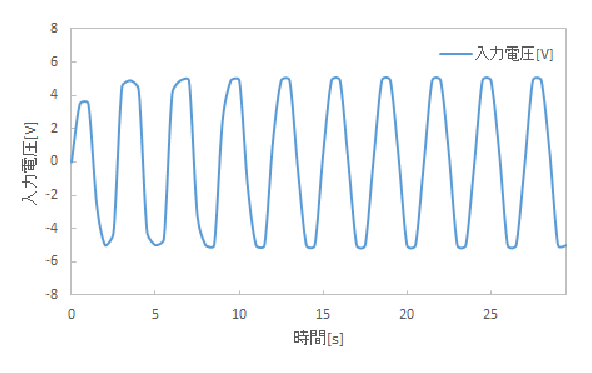
\includegraphics[scale=.6]{./picture/graph11.eps} \\
  (a)入力電圧 \\
  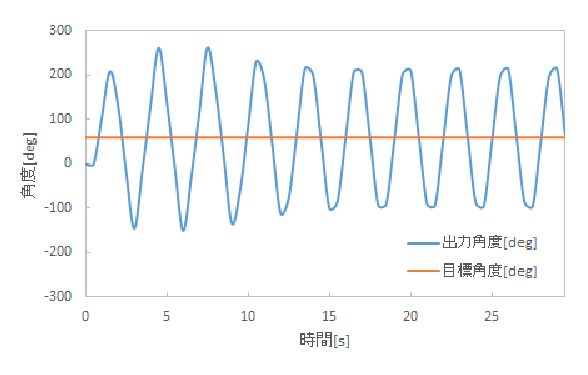
\includegraphics[scale=.6]{./picture/graph12.eps} \\
  (b)角度
  \caption{定数ゲイン2.1,サンプリング周期0.5[s]のときの実験結果}
  \label{fig8}
 \end{center}
\end{figure}


\newpage
\pagestyle{fancy}
\setcounter{page}{1}
\setcounter{section}{1}
\setcounter{figure}{0}
\renewcommand{\thepage}{$再$\,\arabic{page}}
\renewcommand{\headrulewidth}{0.0pt}
\rhead{\thepage}
\lhead{}
\cfoot{}

\section{原理}
本実験で用いる制御系の構成を図\ref{fig1}に示す.

\begin{figure}[b]
 \begin{center}
  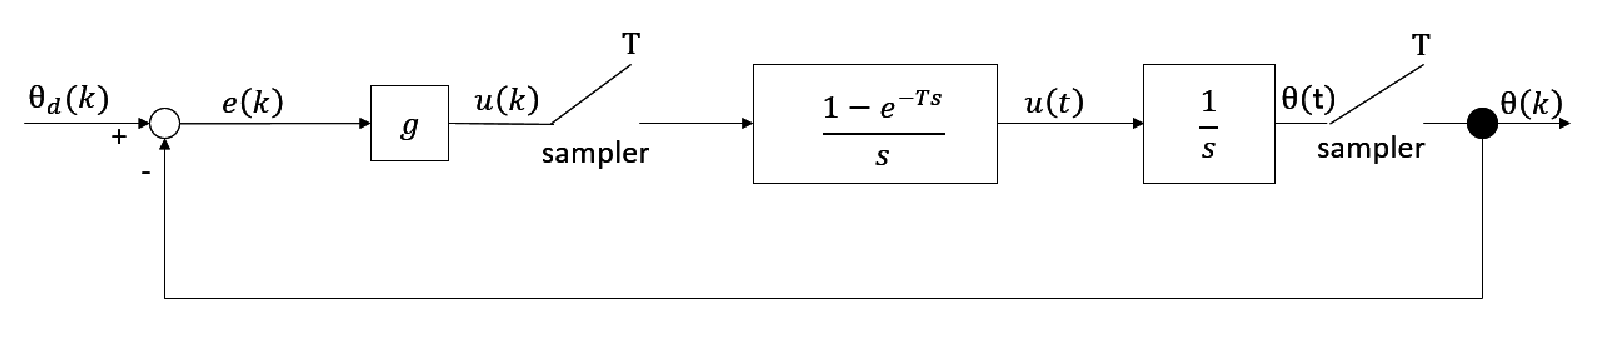
\includegraphics[scale=.6]{./picture/5-blocks2.eps} 
  \caption{制御系の構成}
  \label{fig1}
 \end{center}
\end{figure}

\setcounter{section}{3}

\section{結果と考察}
得られたグラフを図2から図7に示す.
\begin{figure}[b]
 \begin{center}
  \includegraphics[scale=.6]{./picture/regraph1.eps} \\
  (a)入力電圧 \\
  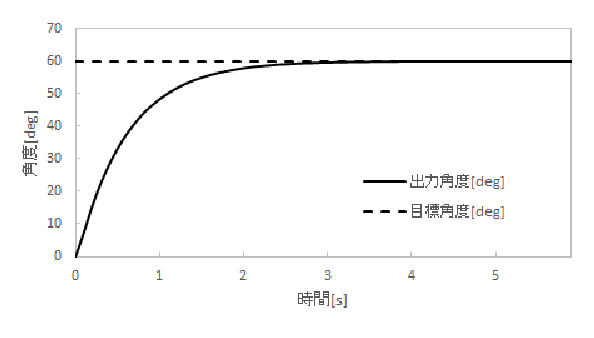
\includegraphics[scale=.6]{./picture/regraph2.eps} \\
  (b)角度
  \caption{定数ゲイン1.0,サンプリング周期0.02[s]のときの実験結果}
 \end{center}
\end{figure}


\begin{figure}[H]
 \begin{center}
  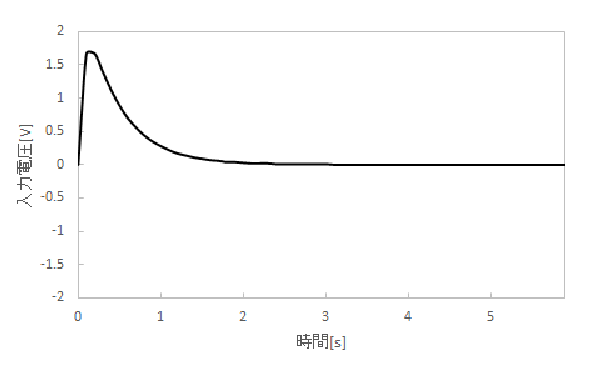
\includegraphics[scale=.6]{./picture/regraph3.eps} \\
  (a)入力電圧 \\
  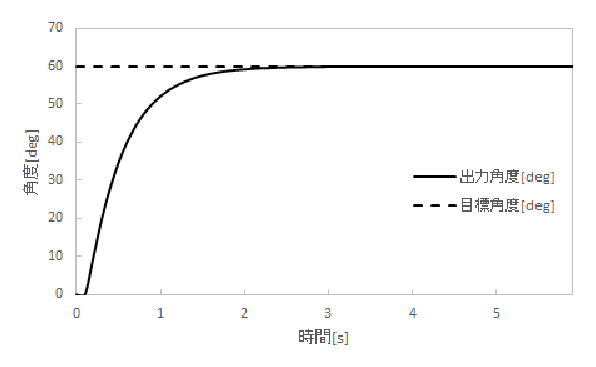
\includegraphics[scale=.6]{./picture/regraph4.eps} \\
  (b)角度
  \caption{定数ゲイン1.0,サンプリング周期0.1[s]のときの実験結果}
 \end{center}
\end{figure}


\begin{figure}[H]
 \begin{center}
  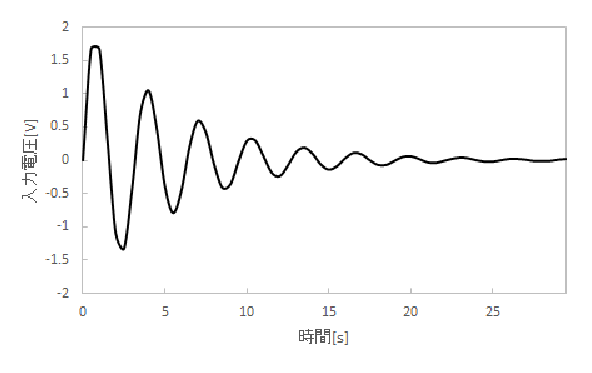
\includegraphics[scale=.6]{./picture/regraph5.eps} \\
  (a)入力電圧 \\
  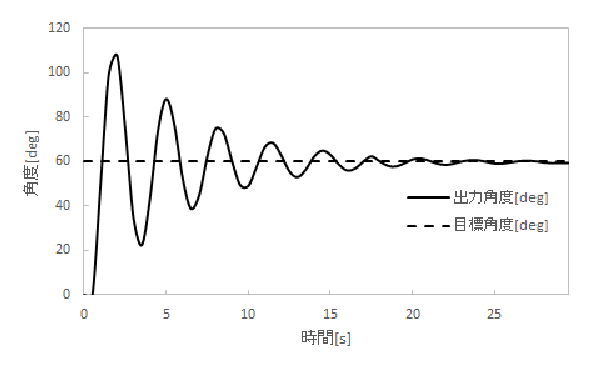
\includegraphics[scale=.6]{./picture/regraph6.eps} \\
  (b)角度
  \caption{定数ゲイン1.0,サンプリング周期0.5[s]のときの実験結果}
 \end{center}
\end{figure}


\begin{figure}[H]
 \begin{center}
  \includegraphics[scale=.6]{./picture/regraph7.eps} \\
  (a)入力電圧 \\
  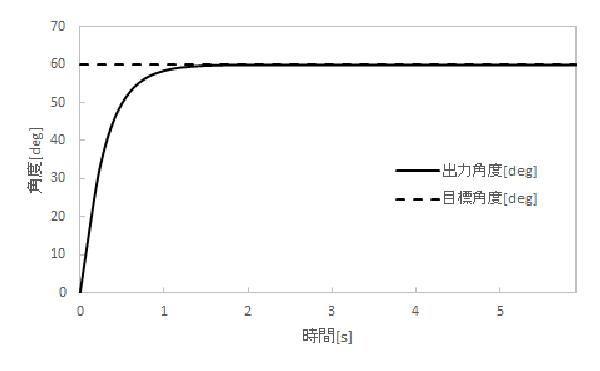
\includegraphics[scale=.6]{./picture/regraph8.eps} \\
  (b)角度
  \caption{定数ゲイン2.1,サンプリング周期0.02[s]のときの実験結果}
 \end{center}
\end{figure}


\begin{figure}[H]
 \begin{center}
  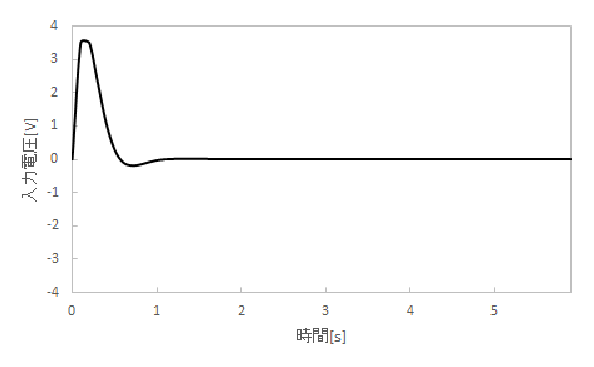
\includegraphics[scale=.6]{./picture/regraph9.eps} \\
  (a)入力電圧 \\
  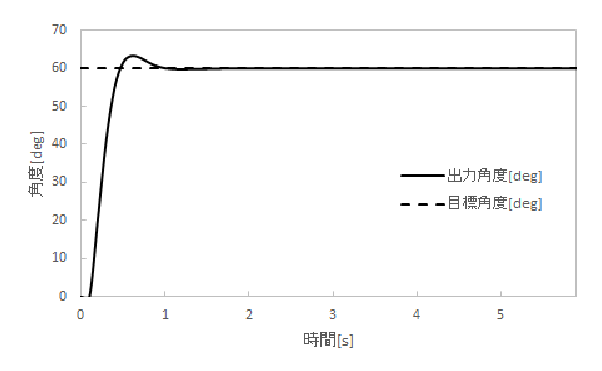
\includegraphics[scale=.6]{./picture/regraph10.eps} \\
  (b)角度
  \caption{定数ゲイン2.1,サンプリング周期0.1[s]のときの実験結果}
 \end{center}
\end{figure}

\begin{figure}[H]
 \begin{center}
  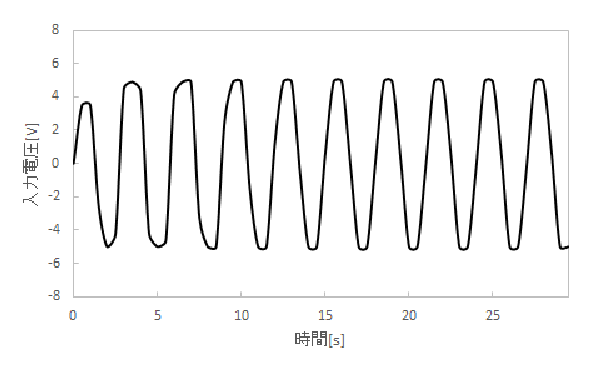
\includegraphics[scale=.6]{./picture/regraph11.eps} \\
  (a)入力電圧 \\
  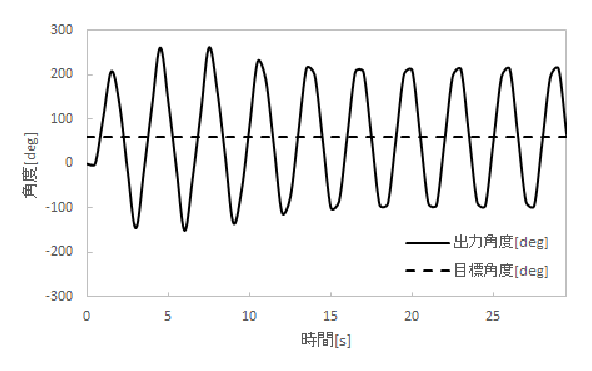
\includegraphics[scale=.6]{./picture/regraph12.eps} \\
  (b)角度
  \caption{定数ゲイン2.1,サンプリング周期0.5[s]のときの実験結果}
 \end{center}
\end{figure}


図2から図2よりそれぞれのときの安定性,立ち上がり時間,整定時間,振動及び行き過ぎの有無を調べると,表\ref{tab7}のようになった.整定時間を求める際の許容誤差を$5\%$とした.

\begin{table}[hb]
 \begin{center}
 \caption{得られたデータから得られた情報}
  \label{tab7}
  \begin{tabular}{|c|c|c|c|c|c|c|c|} \hline
   定数ゲイン & サンプリング周期$T$[s] & $\frac{1}{T}$ & 安定性 & 立ち上がり時間$T_r$[s] & 整定時間$T_s$[s] & 振動 & 行き過ぎ \\ \hline 
      & 0.02 & 50 & 安定   & 1.4 & 1.9 & 無 & 無 \\ \cline{2-8} 
  1.0 & 0.1  & 10 & 安定   & 1.1 & 1.5 & 無 & 無 \\ \cline{2-8}
      & 0.5  & 2  & 安定   &  -  & 17  & 有 & 有 \\ \hline
      & 0.02 & 50 & 安定   & 0.6 & 0.9 & 無 & 無 \\ \cline{2-8}
  2.1 & 0.1  & 10 & 安定   & 0.3 & 0.7 & 無 & 有 \\ \cline{2-8}
      & 0.5  & 2  & 不安定 &  -  &  -  & 有 & 有 \\ \hline
  \end{tabular}
 \end{center}
\end{table}



\subsection{伝達関数の安定性}
式\ref{eq4}より伝達関数の安定性を調べる.この伝達関数の特性方程式は
\begin{equation}
 z^2-x+gT = 0
  \label{eq6}
\end{equation}
次の式よりz平面からs平面へ双一次変換を行う.
\begin{equation}
 z = \frac{s+1}{s-1}
\end{equation}
これを式\ref{eq6}に代入して,
\begin{eqnarray}
 \left( \frac{s+1}{s-1} \right)^2 - \left( \frac{s+1}{s-1} \right)+gT = 0 \nonumber \\ \label{eq8}
 gTs^2 + 2(1-gT)s +2 + gT = 0
\end{eqnarray}
式\ref{eq8}よりフルビッツ行列を用いて安定判別を行う. \\
まず,安定条件は
\begin{eqnarray*}
 gT > 0,2(1-gT) > 0
\end{eqnarray*}
また,フルビッツ行列より
\begin{eqnarray*}
\mathrm{det} \left|
	      \begin{array}{ccc}
	       2(1-gT) &     0   \\
	          gT   &   2+gT  \\
	      \end{array}
	     \right| > 0 \\
 (1-gT)(2+gT) > 0 \\
 g < \frac{2}{T}
\end{eqnarray*}
以上の条件から,伝達関数の安定条件は
\begin{eqnarray*}
 0 < g < \frac{1}{T}
\end{eqnarray*}
となる.

\subsection{定数ゲインとサンプリング周期の変化による実験結果の変化}
この制御系は2次遅れ系であり,定数ゲインを大きくすれば立ち上がり時間は短くなる.また,グラフよりサンプリング周期が長い方が立ち上がり時間が短くなっていることがわかる.


\newpage
\pagestyle{fancy}
\setcounter{page}{1}
\setcounter{section}{4}
\setcounter{figure}{0}
\renewcommand{\thepage}{$再々$\,\arabic{page}}
\renewcommand{\headrulewidth}{0.0pt}
\rhead{\thepage}
\lhead{}
\cfoot{}


\section{考察}
\subsection{極配置による安定判別}
伝達関数の極の実数部分が複素平面上で全て負であれば安定となる.
式8よりこの伝達関数の極は
\begin{equation}
 s = \frac{-(1-gT) \pm \sqrt{1-4gT}}{gT}
\end{equation}
となる.$gT > 0.25$のとき,平方根の項が虚部となる.このとき,伝達関数が安定となるのは
\begin{eqnarray*}
 1-gT & > & 0 \\
 g & < & \frac{1}{T}
\end{eqnarray*}
である.$0 < gT < 0.25$のときは
\begin{eqnarray*}
 -(1-gT)+\sqrt{1-4gT} & < & 0 \\
 1-gT & > & \sqrt{1-4gT} \\
1-2gT+(gT)^2 & > & 1-4gT \\
g & < & \frac{2}{T}
\end{eqnarray*}
となる.よって,安定条件は$0 < g < \frac{1}{T}$である.

\subsection{定数ゲインとサンプリング周期の変化による実験結果の変化}
式4より
\begin{equation}
 \Theta(z) = \frac{gT}{z^2-z+gT} \frac{rz}{z-1}
\end{equation}
これを逆z変換する.
\begin{eqnarray*}
Z^{-1}[\Theta(z)] & = & r\sum_{k = 0}^n g(k)
\end{eqnarray*}
$g(k)$について考えると
\begin{eqnarray}
 \frac{G(z)}{z} & = & \frac{rgT}{(z^2-z+gT)z} \nonumber \\
 & = & \frac{rgT}{(z+1+\sqrt{1-4gT})(z+1-\sqrt{1-4gT})z} \nonumber \\
 & = & rgT \left( \frac{2\sqrt{1-4gT} + 2 - 8gT}{z+1+\sqrt{1-4gT}} 
               - \frac{2\sqrt{1-4gT} - 2 + 8gT}{z+1+\sqrt{1+4gT}} 
               + \frac{4gT}{z} \right)
\end{eqnarray}
ここで,
\begin{equation}
 G(z) = rgT \left( \frac{a_1}{1 + b_1 z^{-1}} - \frac{a_2}{1 + b_2 z^{-1}} + 4gT \right)
\end{equation}
と置くと,
\begin{equation}
 g(k) = rgT(a_1 b_1^k u_s(k) + a_2 b_2^k u_s(k) + \delta(k))
\end{equation}
となる.また,
\begin{eqnarray*}
 a_1 & = & 2\sqrt{1-4gT} + 2 - 8gT \\
 a_2 & = & 2\sqrt{1-4gT} - 2 + 8gT \\
 b_1 & = & 1+\sqrt{1-4gT} \\
 b_2 & = & 1+\sqrt{1+4gT}
\end{eqnarray*}
である.これより,ゲイン$g$を大きくすると$\theta(k)$の各項の値は大きくなるので立ち上がり時間が短くなる.また整定時間も短くなる.同様にサンプリング周期$T$が大きくなれば立ち上がり時間,整定時間が短くなる.しかし,サンプリング周期$T$は大きくしすぎると安定条件を外れてしまう.また,実験で得られたグラフからゲイン$g$が大きいと振動しやすくなることがわかる.よって,どちらも大きすぎず小さすぎない値に設定するべきである.

\begin{thebibliography}{2}
 \bibitem{} 高橋,``ディジタル制御'',岩波書店,1985.
 \bibitem{} 足立,``'信号・システム理論の基礎',コロナ社,2014.
\end{thebibliography}


\end{document}